% Chapter 4

\chapter{实验与分析}
\section{实验环境}
\subsection{模型训练环境}
服务器环境,操作系统为
Ubuntu 16.04.6 LTS (GNU/Linux 4.4.0-142-generic x86\_64),使用命令行ssh工具登入。

内存64GB,搭配显卡2080 Ti 四块,由于资源分配原因本设计中实验使用两块。

使用anaconda 创建虚拟环境,为算法各自安装需要的依赖包与训练环境。
\subsection{软件样本运行环境}
Macbook Pro电脑 15.6寸屏幕版,mid-15 release,A1398型号;
OS X 10.12(Serrina High)系统;
集成显卡,内存16G,没有特别要求。

\section{图片标注实验}
\subsection{模型代码}
模型主题使用了开源代码,由第三方代码作者完成,在Github网站上开源;同时我在其中做了修缮维护,保证了复现在当前版本的依赖包上和现在可以运行的系统里仍然可以运行。

原代码开发环境是python 2.7和tensorflow 0.14,由于目前科学计算使用的python以python3为主流,我将其修改维护至了python 3.6和tensorflow 1.14版本下可以运行的代码。

代码结构分为几个部分:主函数、基本模型类、训练算法。
\subsection{运行过程}
通过在论坛上调研、向专家咨询,我认为较少的数据会导致图片标注模型的效果减弱,会限定构图、限定主题、限定语汇,且识别精确度会很差。为此,我选用了MSCOCO数据集作为训练和测试集。对于这次实验,我先选择了最早的COCO2014数据集,作为试验,后来发现训练时间成本较长,决定使用COCO2014数据集下训练生成的模型作为应用模型。

这一算法的虚拟实验环境python版本为3.7,tensorflow版本为1.14.0,其中安装的依赖包有:numpy 1.17.2,OpenCV 4.1.1.26,NLTK 3.4.5,Pandas 0.25.1,Matplotlib 3.1.1,tqdm 4.36.1。
其中NLTK用作训练集中文字信息的分词处理,仅仅执行了nltk.download("punkt"),作为数据支撑,没有下载完整数据。

模型的训练在实验环境下使用4块NVIDIA 2080 Ti显卡,训练了233小时,执行了100个epoch,每一个epoch都遍历了训练集中的所有数据。

\subsection{遇到的主要问题与解决方法}
\subsubsection{数据传输问题}
服务器的物理地址在浙江大学,属于教育网的浙江位置,从我的工作地点到浙江大学校内当前跳转节点较多,使用RVPN进行连接后,数据传输速度上限是2.00Mbits/sec,所以传输一个总大小为19GiB以上的数据集,需要的时间为40000秒,相当于十余小时。另外,由于RVPN的连接不稳定,而scp命令传输文件不支持断点续传,所以经常出现文件损坏的现象。

经过多次尝试和实践,我采用分包的方式,将数据集化为1GiB到2GiB大小的压缩包,由scp命令逐一传输;同时使用完善、成熟的数据集,尽量最大化一次成功率。

\subsubsection{依赖包函数不兼容问题}
tensorflow在目前的稳定版本中,已经增加了很多新的借口,而1版本和0版本的接口,有一些已经取消了。即使我安装的是1版本的tensorflow环境,仍然有一些接口无法调用。经过调研,我使用了评价较高的tensorflow.compat.v1库,来实现变易出错的接口,解决了大部分问题。

\section{自然语言生成图片实验}
\subsection{模型代码}
模型使用了开源代码,由论文原作者完成,在Github网站上开源;同时我在其中微调,以适合我所需的数据集。

这一套代码的特点是,它含有一套下载数据集的bash代码,方便下载。这一套代码推荐在googleapis.com网站上直接使用wget命令下载数据,这样下载的数据传输速度比较稳定,可以正常下载使用数据。

代码主要包含一个模型运行的主函数、一个模型类和一个训练模型的方法。除此之外,以面向对象的思想对训练过程中的辨别器$D$等类、双线性插值、图片级联优化网络等方法都单独编码,然后加上工具方法的编码,构成了整个工程。

\subsection{运行过程}
运行中由于代码设计,只使用一块显卡进行训练。

因为显卡的设置问题,不可以同时使用同一块显卡即运行tensorflow模型,又训练pytorch模型,因为如果它们同时运行,不同的容器会导致驱动将所有显存都分配给tensorflow的任务,导致pytorch训练的模型无法正常运行。所以,需要等到上一模型训练完毕,再开始训练这一模型。或者,可以让它们在不同的显卡上运行。这在一定程度上影响了我的时间安排,导致我仅在VG数据集上运行了代码。

在VG数据集上,我使用了代码中编写的“强注意力生成”方法制作的生成模型,得到了一个可以从自然语言自动生成图片的模型。

\subsection{遇到的主要问题与解决方法}
这一模型更加的复杂,并且开源代码仅有pytorch版本的实现。按照要求,为了运行这段代码,需要安装python 3.5下的pytorch 0.4.0版本。但是,按照版本要求,在目前的cuda 版本为10.0的电脑中不可以安装这一版本的pytorch了,所以可以替代性地使用torch 1.0.0来运行程序。

在安装虚拟环境的时候,需要注意无论是anaconda官网默认源还是清华大学镜像源都难以链接,并正常下载完毕torch安装包,因为其大小高达700MB,在下载到一半的时候就常常会出现HTTP:200错误代码,导致下载中断。可以打出下列shell命令,将在官网下载好的whl文件安装在环境里。这里的包一定要符合环境下的python版本要求,不知道要求的可以在python shell中运行“wheel.pep425tags. get\_supported()”代码,查询wheel安装要求。

        \text{conda create venv env\_name}

        \text{conda activate env\_name}

        \text{pip\ install\ torch-x.x.x-cp3x-cp3xm-ostype.whl}

        \text{pip\ install\ torchvision}

\section{实验分析与总结}
\subsection{图片标注表现}
对图片标注的模型,我选取了三个模型作为对比,使用BLEU评分\upcite{papineni2002bleu}(Bilingual Evaluation Understudy)的方式进行评价。

BLEU评分是IBM出品的机器翻译评分标准,按照式\eqref{eq:bleu}的算法得出评分。这个评分是对一条翻译打出,后续数据中取平均得分。
\begin{equation}
    \begin{aligned}
        &&BLEU &= &BP \cdot \exp(\sum_{n=1}^N wn\log P_n) \\
        &&\text{其中, }BP&=
        &1 \hspace{9em}& c>r \\ && & &e^{1−r/c}\hspace{7.2em}&c<=r
    \end{aligned}
    \label{eq:bleu}
\end{equation}
式中$BP$即简短惩罚,即在句子短的时候降低评分。在本次评分中,不加入$BP$机制。

其中,我希望测试二十个epoch量级的训练是否可以支撑一个可用的模型,事实上19个epoch的模型经过个例测试,不能很好地生成注意力转移的机制,导致句子不够通顺,经常出现连续无意义重复关键词的现象。后来,我使用这一断点“214999.npy”(后称“断点模型”)继续训练,得到了100个epoch后生成的“289999.npy”(后称“强注意力模型”)模型。

另外,我引入了预训练的“弱注意力模型”的测试数据\upcite{xu2015show},作为对照,观察注意力机制对标注结果的影响,以选取最合适的模型,嵌入软件。对于上述三种模型,我使用nltk包中所带算法,使用1-4精度修正的四种评分进行评价,得到的结果如表所示。其中若关注模型和第二组强关注模型是文献\cite{xu2015show}中的结果。

\begin{table}[!htbp]
    \centering
    \caption{三种模型的BLEU评分}
    \label{tab:bleu}
    \begin{tabular}{cccccc}
        \toprule
        模型选择& BLEU-1 & BLEU-2& BLEU-3& BLEU-4 & METEOR\\
        \hline
        断点模型  & & & & &——\\
        弱关注模型 & 70.7\%&49.2\%&34.4\%&24.3\%&\textbf{23.90\%}\\
        强关注模型(我的训练)&70.3\% &\textbf{53.6\%}&\textbf{ 39.8\%}&\textbf{29.5\%}&——\\
        强关注模型(文中数据)& \textbf{71.8\%}&50.4\%&35.7\%&25.0\%&23.04\%\\
        \bottomrule
    \end{tabular}
\end{table}

可以看到,弱关注模型表现稍好于强关注模型,但是在原文中结论有所不同。因为我自己训练的数据可能因为环境不同表现有少许的差异,但是在同一环境下,强关注模型的训练结果更有利翻译的准确性。

\subsection{文本生成图像算法表现}
理解文本生成的图像涉及到图像标注这一不成熟且复杂度高的算法(正如前文工作所说),所以这一算法的表现不能使用BLEU评分来评价。对于这一图片是否被人理解,采用两种方法评价。

第一种是采用检查图片平滑性的一种评分\upcite{salimans2016improved}(Inspection Scores),作为量化的参考,检查图片质量。这一部分我摘取了StackGAN\upcite{zhang2017stackgan}的相关数据,对比这一算法所生成的图片质量是否过关。从表~\ref{tab:img2txt_1}中可以看出,这一模型所生成的图像在数据上不比StackGAN更加逼真。

\begin{table}[!htb]
    \centering
    \caption{图片平滑性评分与StackGAN模型对比}
    \label{tab:img2txt_1}
    \begin{tabular}{ccc}
        \toprule
        \multirow{2}{*}{模型类别} & \multicolumn{2}{c}{数据集类别}\\
        \cline{2-3}
        &COCO &VG\\
        \hline
        文中模型(无$D_{img}$作用)\upcite{Johnson_2018} &$5.6\pm 0.1$ &$\mathbf{5.7\pm 0.3}$\\
        文中模型 &$6.7\pm 0.1$\upcite{Johnson_2018}&$5.5\pm 0.1$\\
        StackGAN\upcite{zhang2017stackgan}&$\mathbf{8.4\pm 0.2}$&-\\
        \bottomrule
    \end{tabular}
\end{table}

第二种评价方法是主观评价,具体观看例句生成的图片,感受图片质量的差别。在Github开源代码中可以找到StackGAN模型的预训练模型\footnote{在github网址 https://github.com/hanzhanggit/StackGAN-Pytorch 可以找到预先训练完成的模型,并从原文找到了评测数据},可以根据这一模型用测试语句生成图像,对比直观效果。

\begin{figure}[!htb]
    \centering
    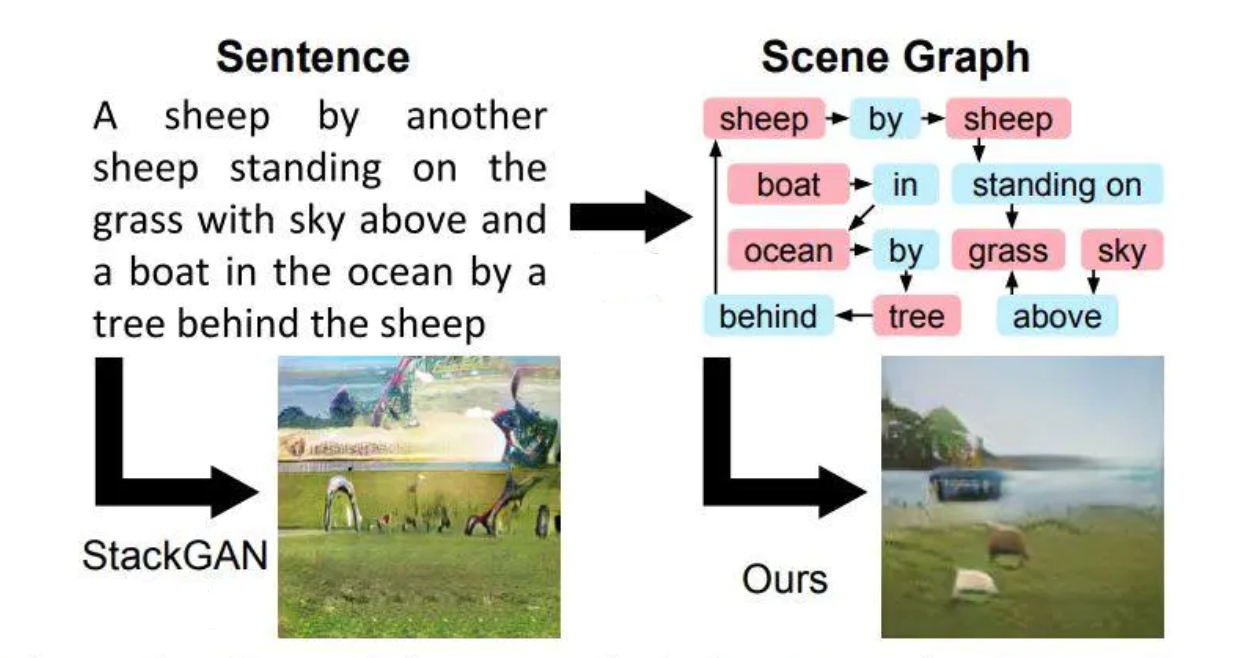
\includegraphics[width=0.8\textwidth]{figures/sg2imcp.png}
    \caption{比较StackGAN和本文算法的生成图像差异}
    \label{fig:sg2imcp}
\end{figure}

有一首小诗\footnote{由文献\cite{Johnson_2018}原作者提出,以解释模型在生成图像方面的优势},因为其包含许多位置关系,非常适合这一算法。以此为例,可以表现此算法对人类主观理解上的优势。

对于如下诗句,StackGAN模型和本文使用模型分别生成了如图~\ref{fig:sg2imcp}的两张截然不同的图像。显然,本文使用模型保留了大部分的位置关系,并且没有产生图像上的扭曲。从人类的视角来看,

A sheep by another sheep

standing on the grass

with sky above and a boat in the ocean

beyond the tree next to the sheep.

另外,在图~\ref{fig:sg2imeg}我们可以清晰地从场景关系图的树状发展流程中,看到构成生成图片的过程。

\begin{figure}[!htbp]
    \centering
    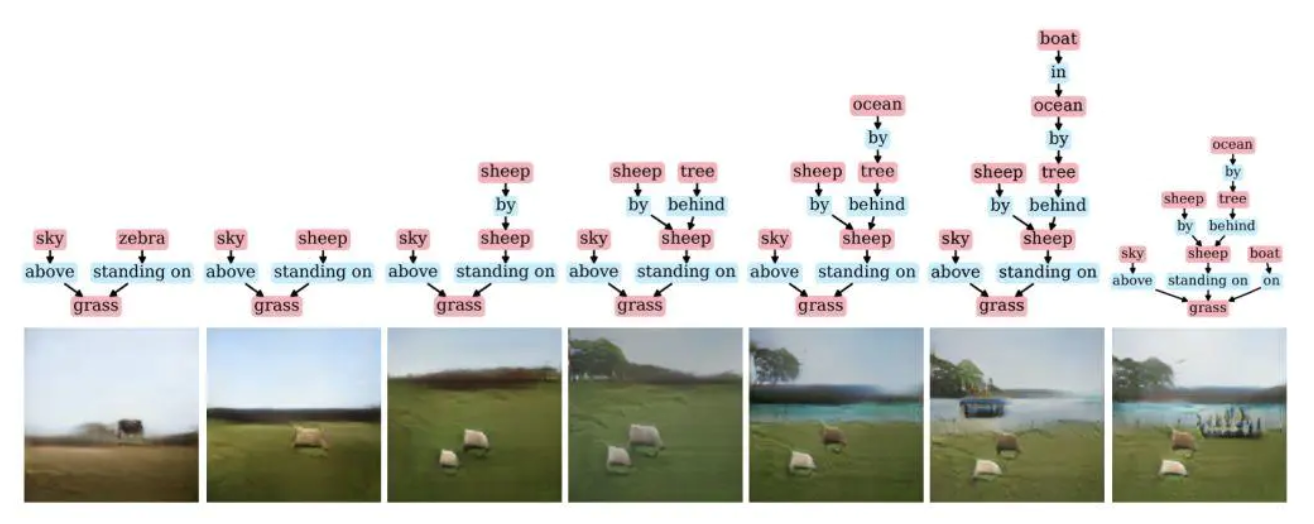
\includegraphics[width=0.8\textwidth]{figures/sg2imeg.png}
    \caption{比较StackGAN和本文算法的生成图像差异}
    \label{fig:sg2imeg}
\end{figure}

\section{本章小结}
这一章节分别介绍了软件界面编码方式、软件两个功能模型训练方式过程与软件部署调试的过程。在软件界面编码中,试用了tkinter进行编码,用比较简明的方式,实现了用例图中的效果;在软件功能模型训练中,记述了LSTM模型和GAN模型分别在环境安装、数据集选取、训练次数调整和呈现方式的过程

%{\songti \bfseries 宋体加粗} {\textbf{English}}

%{\songti \itshape 宋体斜体} {\textit{English}}

%%%{\songti \bfseries \itshape 宋体粗斜体} {\textbf{\textit{English}}}

%\section{编译}
%本模板必须使用XeLaTeX + BibTeX编译,否则会直接报错。 本模板支持多个平台,结合sublime/vscode/overleaf都可以使用。